\chapter{Frontend}

While I had the option of writing pure JavaScript, because this is an application of a larger scale than I am used to I knew that with a dynamically typed language such as JavaScript the project will be harder to maintain as it grows, as a result I much more preferred TypeScript. I wrote type annotations everywhere I could. In retrospective this was one of the best decisions I made, I have avoided type errors that would have taken a long time to discover and the development experience was great thanks to code hinting tools available in IDEs\footnote{Integrated development environments}.

Observant people might have noticed that the application respects the Material Design\footnote{\href{https://material.io/design}{https://material.io/design}} guidelines, this is not because I created the components myself to respect the design system but because I chose to use a component library (React Material-UI\footnote{\href{https://www.npmjs.com/package/@material-ui/core}{https://www.npmjs.com/package/@material-ui/core}}) that has built-in styling and much more. As a consequence a consistent user interface was achieved, and more importantly a significant amount of developing time was saved due to not having to fiddle with styling or writing boilerplate code, all while reusing robust components that respect semantic markup.

Wherever I had to write components I tried my best to organise them into two categories: 
\begin{itemize}
	\item Smart components - these components maintain state, perform operations on data and they don't have anything to do with view logic, they simply pass the necessary data to the dumb components
	\item Dumb components - in contrast, these components' sole purpose is to present the data
\end{itemize}

Going further I am going to detail the organization of the files and directories, then I will talk about used conventions and dive deep into some details.

\section{Project structure}

Figure \ref{figure:frontend-project-structure} illustrates the files and directories hierarchy. \textit{buildspec.yml} includes the build specifications, \textit{tsconfig.json} contains the rules regarding transpilation, \textit{.eslintrc.json} is the configuration file for ESLint that enforces code conventions and consistent styling and \textit{.prettierrc.yaml} is the configuration file for the Prettier\footnote{\href{https://prettier.io/}{https://prettier.io/}} code formatter. The application's dependencies are installed under the \textit{node\_modules} directory and as for any web application the static files are found in the \textit{public} directory. In the pages directory each file corresponds to a page in the web application. Looking at the \textit{src} and \textit{pages} directory we observe that they are mirrored in some way, that is because I have opted to organize page components by features instead of by type. This was caused by a refactoring midway through the project for the reason that components organized by type didn't scale well at all. The opted for file structure brought components used in the same context closer together, thus higher cohesion was achieved, for instance components required by the index page belong to the \textit{components/index} directory. The \textit{components/shared} directory is intended for components that can be reused. 

Going into more detail, the \textit{contexts} and \textit{hooks} directories are React oriented. Among the choices I had for managing application state I chose the React Context API because it was the built-in solution for this and so contexts live in the \textit{contexts} directory. Hooks are a way to achieve code reusability and similar to contexts they too exist in their own directory.

\begin{figure}[H]
\begin{verbatim}
FE
|- buildspec.yml
|- tsconfig.json
|- .eslintrc.json
|- .prettierrc.yaml
|- node_modules
|- public/
|- src/
   |- components/
      |- profile/
      |- stages/
      |- forgot-password/
      |- index/
      |- sign-in/
      |- sign-up/
      |- shared/
   |- contexts/
   |- hooks/
   |- pages/
   	  |- profile/
   	     |- change-email.tsx
   	     |- change-password.tsx
   	     |- index.tsx
   	  |- stages/
   	     |- add.tsx
   	     |- edit.tsx
   	     |- index.tsx
   	  |- forgot-password.tsx
   	  |- index.tsx
   	  |- sign-in.tsx
   	  |- sign-up.tsx
   |- types/
   |- utils/
\end{verbatim}
\caption{Frontend project structure.}
\label{figure:frontend-project-structure}
\end{figure}

\section{Used conventions}

As a result of writing dozens of files and components I have established some conventions that helped the arrangement of code inside a file.

\subsection{Absolute imports}

Thanks to a feature available in TypeScript that allows to change module resolution, I could use absolute imports therefore avoiding relative import hell. If it wasn't for this feature there would've been non-comprehensible imports like the following:

\begin{lstlisting}[language=JavaScript]
import { component } from "../../../../../components";
\end{lstlisting}

I have configured the following mapping for imports:

\begin{verbatim}
#public/*     --> public/*
#components/* --> src/components/*
#utils        --> src/utils
#types/*      --> src/types/*
#shared       --> src/shared
#contexts     --> src/contexts
#hooks        --> src/hooks
\end{verbatim}

Therefore, if I had to import a component I would simply type something like:

\begin{lstlisting}[language=javaScript]
import { component } from "#components";
\end{lstlisting}}

As seen above, I chose absolute imports to be prefixed with the \# symbol. At first I chose @ to be the symbol but not too soon after I realized there are npm packages using @ as a prefix and that could lead to potential confusion. The change from @ to \# happened due to a refactor.

\subsection{Order of imports and exports}

In some files there is a long list of imports so I decided to structure them in some way, this can be seen for an example file in Figure \ref{figure:frontend-import-order}. External dependencies are first, followed by absolute imports in the project and relative imports. By examining a significant amount of files I found the relative imports to have depth at most two, so relative import hell is avoided. I think that this import order convention greatly improves legibility.

\begin{figure}[H]
\begin{lstlisting}[numbers=left,language=JavaScript]
import React, { useContext } from 'react';
import { CognitoUserSession } from 'amazon-cognito-identity-js';
import { Socket } from 'socket.io-client';
import { Emitter } from 'mitt';
import axios from 'axios';
import { Container, Paper } from '@material-ui/core';
import { translateMessage } from '#utils';
import { AccountContext, SocketContext } from '#contexts';
import type { MessageType } from './shared';
import ChatHeader from './chatHeader';
import ChatBody from './chatBody';
import ChatFooter from './chatFooter';
import { AttenderType } from '../stage/shared';
\end{lstlisting}
\caption{Frontend import order convention.}
\label{figure:frontend-import-order}
\end{figure}

I have established a convention about exports as well, they are always placed at the end of the file so whenever somebody wants to see what a file exports they only have to look at the end of it.

\section{Deep dive}

In think section we will go in-depth about certain functionalities that I consider to be important.

\subsection{Forms with validation}

While building the pages required for authentication I found value in building reusable components that performed input validation. In doing so my tools of choice were Formik\footnote{Easier React form validation: \href{https://www.npmjs.com/package/formik}{https://www.npmjs.com/package/formik}} and Yup\footnote{Schema builder: \href{https://www.npmjs.com/package/yup}{https://www.npmjs.com/package/yup}} which I have augmented in order to abstract and generalize input fields and their validation. In figures \ref{figure:frontend-validation-schema} and \ref{figure:frontend-sign-up-form} are snippets of code that showcase how the fields in the sign up page are handled, namely Figure \ref{figure:frontend-validation-schema} is the object schema the fields in the form have to respect and Figure \ref{figure:frontend-sign-up-form} is the code for the form without boilerplate code in order to increase brevity.

\begin{figure}[H]
\begin{lstlisting}[numbers=left,language=JavaScript]
const validationSchema = Yup.object().shape({
  firstName: Yup.string().required('Your first name is required.'),
  lastName: Yup.string().required('Your last name is required.'),
  email: Yup.string()
    .email('Invalid email format.')
    .required('Your email is required.'),
  password: Yup.string()
    .min(8, '8 characters minimum.')
    .matches(/\d/, 'A number is required.')
    .required('A password is required.'),
  passwordConfirm: Yup.string()
    .oneOf([Yup.ref('password'), null], 'Passwords must match.')
    .required('Password confirm is required.'),
});
\end{lstlisting}
\caption{Frontend validation schema example.}
\label{figure:frontend-validation-schema}
\end{figure}

Notice in Figure \ref{figure:frontend-sign-up-form} on line 1 I pass the validation schema object created earlier. The \verb|FormikField| component I built is responsible for displaying errors in case there are any. With this highly reusable setup I created the forms for the profile page in just a couple hours.

\begin{figure}[H]
\begin{lstlisting}[numbers=left,language=JavaScript]
  <Formik validationSchema={validationSchema}>
        {(props): { props: FormikProps<typeof initialValues> } => (
          <>
              <ChooseAvatar
                email={props.values.email}
                avatarSrc={avatarSrc}
                setAvatarSrc={setAvatarSrc}
              />
              <FormikField type="email" name="email"
              	 label="Email" required />
              <FormikField type="text" name="firstName"
              	 label="First name" required />
              <FormikField type="text" name="lastName"
              	 label="Last name" required />
              <FormikField type="password" name="password"
              	 label="Password" required />
              <FormikField type="password" name="passwordConfirm"
                label="Password Confirm" required />

              <Button
                endIcon={<ArrowForward />}
                variant="contained"
                color="primary"
                type="submit"
                disabled={props.isSubmitting}
              >
                Sign up
              </Button>
          </>
        )}
      </Formik>
\end{lstlisting}
\caption{Frontend simplified sign-up form code.}
\label{figure:frontend-sign-up-form}
\end{figure}

\subsection{3D stage}

One of the more interesting areas of the application is the 3D stage available at the index page. Instead of using the WebGL\footnote{Web Graphics Library: \href{https://developer.mozilla.org/en-US/docs/Web/API/WebGL_API}{https://developer.mozilla.org/en-US/docs/Web/API/WebGL\_API}} API, which would have meant going extremely in detail with 3D graphics, I picked a popular JavaScript library named Three.js\footnote{\href{https://threejs.org/}{https://threejs.org/}}. One issue I had to deal with was the imperative programming nature of this library and its incompatibility with React, thankfully though multiple people in the same situation as me were inspired to build a wrapper-like library (@react-three/fiber\footnote{\href{https://www.npmjs.com/package/@react-three/fiber}{https://www.npmjs.com/package/@react-three/fiber}}) that provides both the declarative aspect of React and the abstractness of working with 3D of Three.js. The advantage was that code could be organized in React components, unfortunately in some situations imperative code had to be written because there was no other choice to achieve certain functionality.

Because the code that contains the logic for rendering the 3D scene is filled with intricacies of the libraries I used I am going to give a high level explanation instead. I will describe each component of the 3D scene:

\begin{itemize}
	\item \verb|StageFloor| component - consists of the "walking area" where the attendees are moving on, its geometry is a box and its material has attached a dark wood-like texture. It is responsible for intercepting clicks by the use of ray casting and for adding the arrow object as a visual feedback for clicking. It also transmits the coordinates of where the casted ray intersected via an event to the \verb|AttenderManager| component.
	\item \verb|Wall| component - this is the simple background sitting behind the playing video, it has a box geometry and a white material texture.
	\item \verb|Screen| component - the plane where the media is seen, the component receives a link to a video or image and fallbacks to a generic image in case none of the provided links point to a valid source. It is responsible for muting and unmuting the video sound when it is clicked.
	\item \verb|AttenderManager| - this component deals with showing the avatars of the attendees in a stage, it communicates with the backend server in order to receive position changes and other user data.
\end{itemize}

\subsection{Chat component}

The \verb|ChatManager| component handles the chat functionality. It communicates with the backend using websockets and with S3 directly when photos are sent. It reacts to twelve events in total which can be split into two categories: \textbf{local emitted} events and \textbf{server emitted} events. A short description will be given to each one of the events.

The local emitted events are emitted and received by the client, this was used in order to decouple components. The local events are the following: 
\begin{itemize}
	\item \verb|close-chat| - handles the logic when a chat is closed
	\item \verb|opened-chat| - triggered by the \textit{Message} action within a user pop-up, adds and opens the new chat
	\item \verb|change-chat| - triggered when a new chat is selected
	\item \verb|private-message| - triggered when a message is sent, it appends a message and sends it to the backend so the message gets delivered to the other chat participant(s)
	\item \verb|file-upload| - triggered when a photo is selected to be uploaded from the file system, it queries the backend for a signed URL with which the client can directly upload the photo to S3
	\item \verb|chat-messages| - triggered when the top of the messages has been reached, it queries the backend for the next page of messages if available
\end{itemize}

The server emitted events are emitted by the backend server and received by the client. The server emitted events are the following:
\begin{itemize}
	\item \verb|put-file-signed-url| - this event occurs only after a locally emitted \verb|file-upload| event, the content of this event is a signed S3 URL which allows data upload
	\item \verb|notifications| - emitted when the user connects and had pending notifications that now need to be shown
	\item \verb|chat-messages| - first the client emits this event to the server, after which the server responds with the event of the same name containing messages of a newly selected chat
	\item \verb|private-message| - emitted by the server when the client has received a new message
	\item \verb|connected-users| - emitted when the user has connected to the chat, receives data about which users are online
	\item \verb|user-state-change| - emitted by the server when a client has connected/disconnected
\end{itemize}

 It is important to specify what data are used here, each chat respects the contract specified by the TypeScript \verb|interface| in Figure \ref{figure:frontend-chatmanager-headerchat}. The \verb|UserAttributes| interface is shown in Figure \ref{figure:frontend-chatmanager-userattributes}. The fields suffixed by a question mark are optional, some fields were eliminated in order to increase brevity.

So, each chat contains how many notifications there are from a user, whether that user is online or not, whether that chat is the current selected one and a lot of information about the user in question. The reason for holding all the information specified by the \verb|UserAttributes| contract about a user is in order to get fast access to more information about that user, so no additional lengthy network requests are made.

\begin{figure}[H]
\begin{lstlisting}[numbers=left,language=JavaScript]
interface HeaderChatType {
  user: UserAttributes;
  notifications: number;
  online: boolean;
  selected: boolean;
}
\end{lstlisting}
\caption{Format of the information of a chat.}
\label{figure:frontend-chatmanager-headerchat}
\end{figure}

\begin{figure}[H]
\begin{lstlisting}[numbers=left,language=JavaScript]
interface UserAttributes {
  picture: string;
  id: string;
  email: string;
  emailVerified: boolean;
  givenName: string;
  familyName: string;
  groups?: string[];
  roles?: string[];
  preferredRole?: string;
  customFacebook?: string;
  customLinkedin?: string;
  customPhone?: string;
  customJob?: string;
  customLanguage?: string;
}
\end{lstlisting}
\caption{Format of the information of a user.}
\label{figure:frontend-chatmanager-userattributes}
\end{figure}

For the actual messages exchanged in the chat, the formats of the data are those shown in Figure \ref{figure:frontend-chatmanager-message}. Here we don't store so much information about the user and a network request has to be done if somebody wants to gather more information about the user that sent a message. The justification here is obvious, there would have been simply too much redundant data if all the user information was stored alongside a message.

So, in total, for a message we have the originator's ID so we can obtain more information about him, his name and picture to show in the chat, the MIME type of the sent message so we know what to show on the frontend, the actual data of the message which can be plain text or a link to S3 of the media file uploaded and the time when the message was sent. Additionally, if the message type is plain text, an \verb|ISO-639-1| language code will be attached to the message in order to accomplish the text translation functionality, or if the message contains media it will contain an alternative text describing the image.

\begin{figure}[H]
\begin{lstlisting}[numbers=left,language=JavaScript]
type UserInformationType = {
  id: string;
  name: string;
  picture: string;
};

interface BaseMessage {
  userInformation: UserInformationType;
  type: string; // MIME type of messages
  data: string;
  time: number;
}

interface TextMessageType extends BaseMessage {
  // ISO-639-1 language code
  language: string;
}

interface MediaMessageType extends BaseMessage {
  // alternative text description of the media
  alt: string;
}
\end{lstlisting}
\caption{Format of a chat message.}
\label{figure:frontend-chatmanager-message}
\end{figure}

Sharp-eyed readers might have noticed that both the \verb|AttenderManager| and \verb|ChatManager| components communicate with the backend, however they are not coupled by any means.

\subsection{Restricting access to protected routes}

Just like a lot of other applications, some routes requires the user to be authenticated. For this I have created a reusable component that wraps the protected component, it allows access if the user is authenticated and it redirects the user to the index page if not. Figure \ref{figure:frontend-require-authentication} shows legible code that can be understood even by those unfamiliar with the used tools and technologies.

\begin{figure}[H]
\begin{lstlisting}[numbers=left]
const RequireAuthentication: React.FunctionComponent = 
  ({ children }) => {
  const router = useRouter();
  const { isLoggingIn, isLoggedIn } = useUser();

  if (isLoggingIn) {
    // loading user state
    return <></>;
  }

  if (!isLoggedIn) {
    // if user is not logged in, redirect to index page
    router.push('/');
    return <></>;
  }

  return <>{children}</>;
};
\end{lstlisting}
\caption{Require authentication reusable component.}
\label{figure:frontend-require-authentication}
\end{figure}

\subsection{Computing language to translate messages to}

Not every user will go to the profile page and change their preferred language, therefore fallbacks had to be implemented in this regard. The function that performs this computation is shown in Figure \ref{figure:frontend-get-user-language}:

\begin{figure}[H]
\begin{lstlisting}[numbers=left,language=JavaScript]
const getUserLanguage = (user) => {
  if (user.customLanguage) return user.customLanguage;
  if (window.navigator.language) return window.navigator
                                          .language.split('-')[0];
  return 'en';
};
\end{lstlisting}
\caption{Function that computes the user language.}
\label{figure:frontend-get-user-language}
\end{figure}

The return value has to be a ISO-639-1 language code, hence the splitting at line 4. The \verb|window.navigator.language| value should be a string representing the preferred language of the user, in case that doesn't exist as the last fallback we choose the english language.


\subsection{Accessibility features}

When clicking on the playing media in the stage, an animation brings the camera closer to the plane whose texture is that of the media. Depending on the device the camera position will cut more or less of that plane, therefore I have applied principles similar to responsive web design by adjusting the camera position based on the width of the page.

Another accessibility feature is dark mode so during night time (or low light conditions in general) the user's eye strain is reduced. The toggle for light/dark mode is found in the rightmost upper right button in the page. Example of how the page looks with it toggled on is shown in Figure \ref{figure:frontend-darkmode}.

\begin{figure}[H]
	\centering
	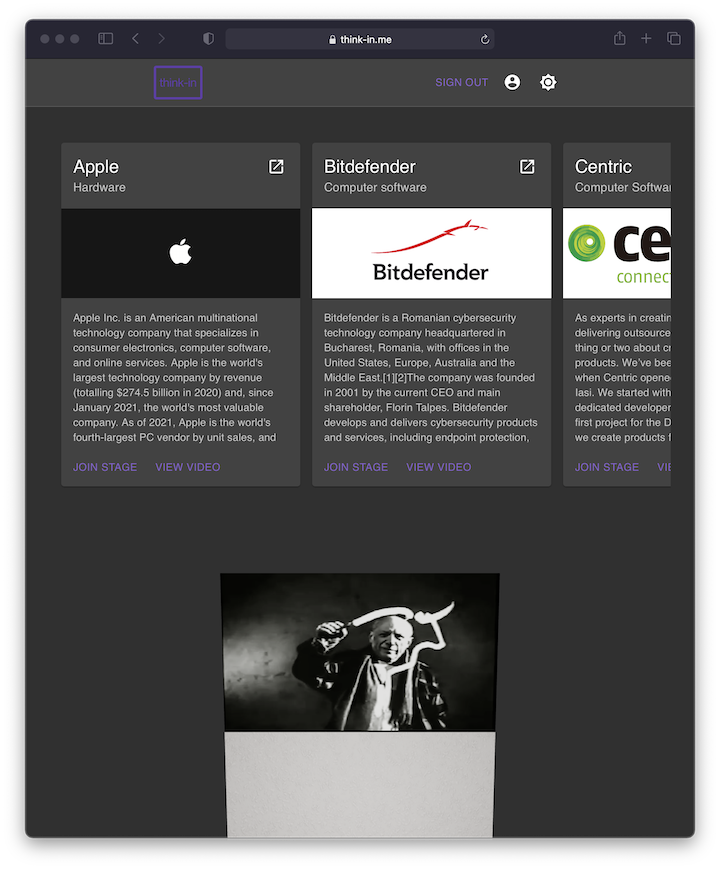
\includegraphics[width=.99\textwidth,keepaspectratio]{images/frontend/darkmode.png}
	\caption{Frontend dark mode.}
	\label{figure:frontend-darkmode}
\end{figure}


Moreover, I have attempted to fix the case where two attendee's avatars are overlapping such as shown in Figure \ref{figure:frontend-overlapping-non-fixed}, here we would have trouble clicking on \textit{User Two}'s avatar because \textit{User One} is sitting right in front of him. One could imagine this could become a real problem when a large amount of people are connected.


\begin{figure}[H]
	\centering
	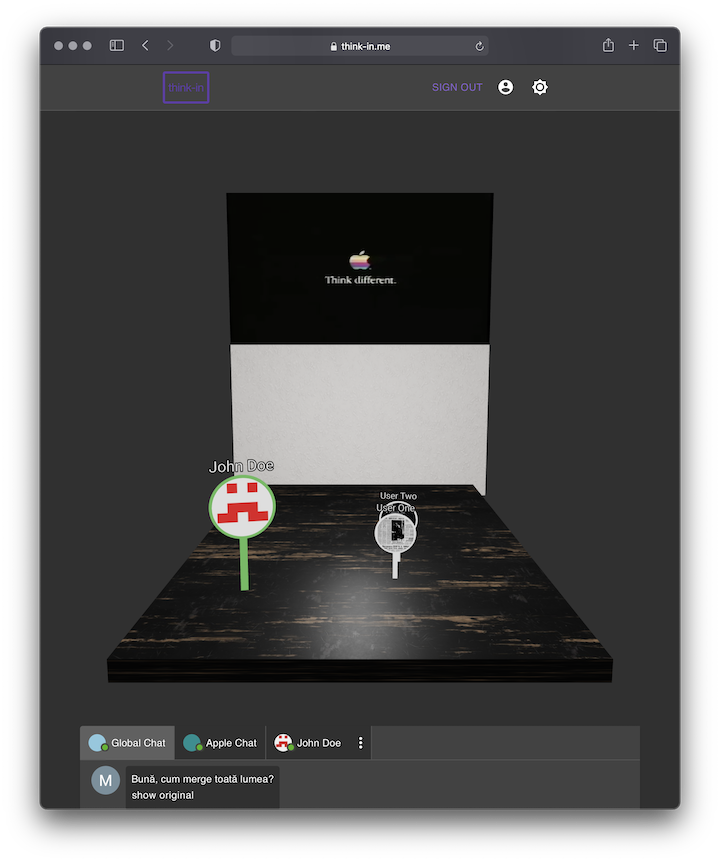
\includegraphics[width=\textwidth,keepaspectratio]{images/frontend/overlapping-non-fixed.png}
	\caption{Overlapping original camera view.}
	\label{figure:frontend-overlapping-non-fixed}
\end{figure}

As an attempt to fix the issue just described I allow the users to control the camera by moving it around the origin as well as zooming in. An example of when a user has moved the camera is shown in Figure \ref{figure:frontend-overlapping-fixed}, here the user has moved the camera just enough in order to see \textit{User One} and \textit{User Two} not overlap anymore.

\begin{figure}[H]
	\centering
	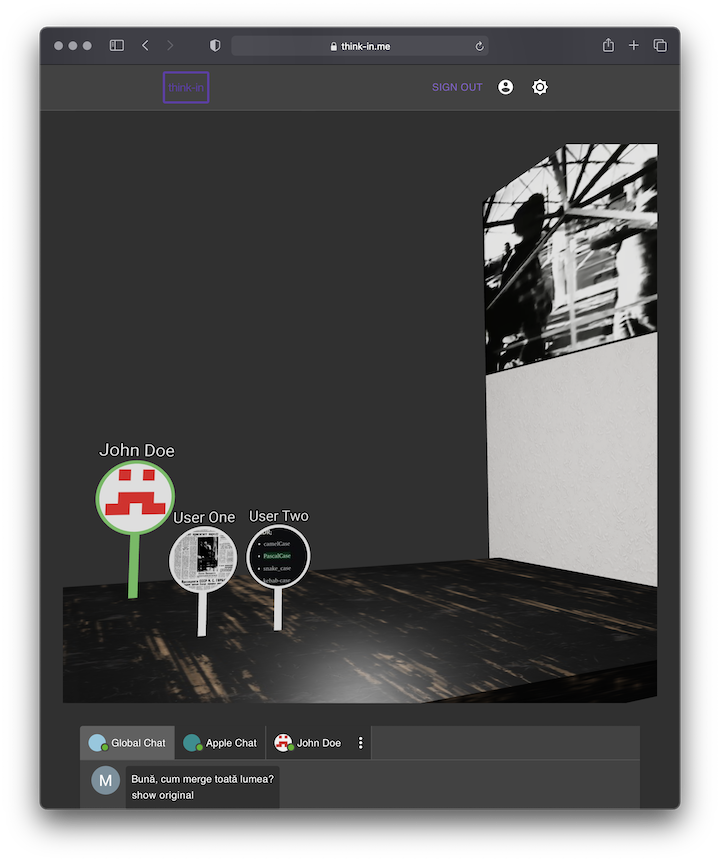
\includegraphics[width=\textwidth,keepaspectratio]{images/frontend/overlapping-fixed.png}
	\caption{Non-overlapping camera view.}
	\label{figure:frontend-overlapping-fixed}
\end{figure}


